\chapter{Компенсирующий регулятор по состоянию}
\label{ch:chap1}
\section{Условие задания}
Рассмотрим систему, состоящую из объекта управления, генератора внешнего возмущения и виртуального выхода:
$$
  \begin{cases}
    \dot{x} = Ax + Bu + B_f w_f, \tab x(0)= \begin{bmatrix} 0 & 0 & 0 \end{bmatrix}^T, \\
    \dot{w_f} = \text{Г}w_f, \tab w_f(0) = \begin{bmatrix} 1 & 1 & 1 & 1 \end{bmatrix}^T \\ 
    z = C_Zx
  \end{cases}
$$ и выполним следующие шаги:

\begin{itemize}
  \item Найти собственные числа матрицы \text{Γ} и определить характер внешнего возмущения.
  \item Построить схему моделирования системы, замкнутой компенсирующим регулятором $u =K_1x+K_2w_f$.
  обеспечивающим выполнение целевого условия $\lim_{t\to +\infty} z(t) = 0$ при внешнем воздействии, задаваемом генератором.
  \item Синтезировать «feedback»-компоненту $K_1$ компенсирующего регулятора. Привести выкладки процедуры синтеза и
  полученную матрицу $K_1$.
  \item Синтезировать «feedforward»-компоненту $K_2$ компенсирующего регулятора. Привести выкладки процедуры синтеза и полученную матрицу $K_2$.
  \item Выполнить моделирование, состоящее из трёх частей.
  \item  Проанализировать полученные результаты и сделать выводы.
\end{itemize}

Начальные данные:

$$
  A = \begin{bmatrix}
    12 & -1 & 14 \\
    6 & 0 & 6 \\
    -6 & -2 & -8 \\
\end{bmatrix}, \tab B = \begin{bmatrix}
  11 \\
  7 \\
  -7 \\
\end{bmatrix}, \tab C = \begin{bmatrix}
  -2 \\ 2 \\ -1 \\
\end{bmatrix}^T, \tab D = \begin{bmatrix}
  6 \\
  -6 \\
  -4 \\
  -5 \\
\end{bmatrix}^T, 
$$
$$
G = \begin{bmatrix}
  -40 & 16 & 9 & -7 \\
  -64 & 25 & 14 & -12 \\
  -26 & 11 & 7 & -3 \\
  48 & -18 & -14 & 8 \\
\end{bmatrix}, \tab B_f =\begin{bmatrix}
       0 & 2 & -1 & 0 \\
       0 & 0 & 0 & 0 \\
       0 & -2 & 0 & 0 \\
   \end{bmatrix}, \tab
  C_Z = \begin{bmatrix}
    2 \\ 1 \\ 3 \\
\end{bmatrix}^T
$$


\section{Решение задания}

Найдём собственные числа матрицы \text{Г}:
$$
  \sigma(\text{Г}) = \{ \pm 3i, \pm 2i \}
$$
Определим характер внешнего возмущения, восстановив его по модам выше:
$$
  w_f(t) = sin(3t) + cos(3t) + sin(2t) + cos(2t) = \sqrt{2}( sin(2t  + \frac{\pi}{4}) + sin(3t + \frac{ \pi}{4}) )
$$
Таким образом внешние возмущения представляют гармонические сигналы с частотой $\omega = 2$ и $\omega = 3$.

Построим схему моделирования системы, замкнутой компенсирующим регулятором $u =K_1x+K_2w_f$. В нашем случае мы решаем задачу компенсации, поэтому наше целевое условие:
$$
  \lim_{t\to +\infty} z(t) = 0
$$
При внешнем воздействии, задаваемом генератором. 
\begin{figure}[ht]
  \centering
  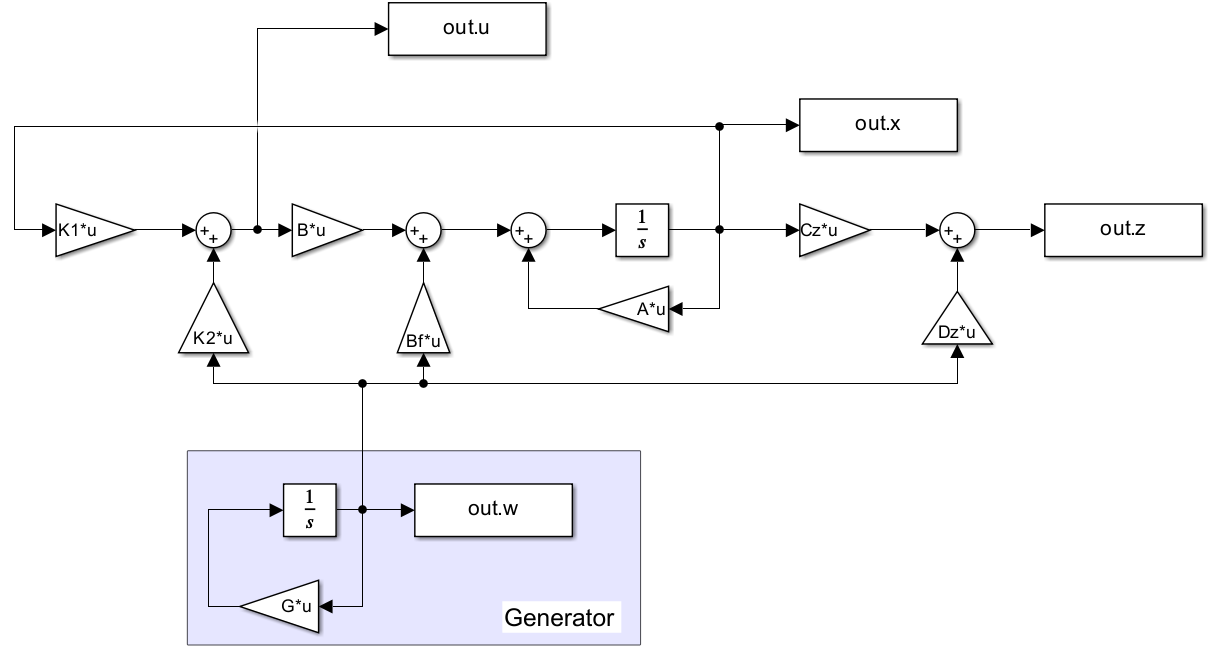
\includegraphics[width=1.0\textwidth]{scheme1.png}
  \caption{Схема - моделирование компенсирующего регулятора по состоянию}
\end{figure}

Синтезируем «feedback»-компоненту $K_1$ с помощью \text{LQR}-регулятора, функционал качества:
$$
  J = \int_0^{\infty} (x^TQx + u^TRu) dt
$$ 
Будем минимизировать при помощи следующих параметров:
$$
  Q = \begin{bmatrix}
    1 & 0 & 0 \\
    0 & 1 & 0 \\
    0 & 0 & 1
  \end{bmatrix}, \quad R = \begin{bmatrix}
    1
  \end{bmatrix}
$$
В результате получаем матрицу $K_1$:
$$
  K_1 = \begin{bmatrix}
    8.71 & -8.62 & 8.47 \\
\end{bmatrix}
$$

Синтезируем «feedforward»-компоненту $K_2$ компенсирующего регулятора, проследуем следующему алгоритму:
\begin{itemize}
  \item Выбрать матрицу $K_1$: $\sigma(A+BK_1)\in\mathbb{C}_{-}$
  \item Найти $P, Y$ как решение системы уравнений:
  
  $$
  \begin{cases}
    PG - AP = BY + B_f \\
    C_Z P + D_Z = 0
  \end{cases}
  $$

  \item Вычислить $K_2$: $K_2 = Y - K_1 P$
\end{itemize}
В результате получаем матрицу второй компоненты регулятора:
$$
  K_2 = \begin{bmatrix}
    8.71 & -8.62 & 8.47 \\
\end{bmatrix}
$$

\newpage
\subsection{Разомкнутая система, $u=0$}

\begin{figure}[ht]
  \centering
  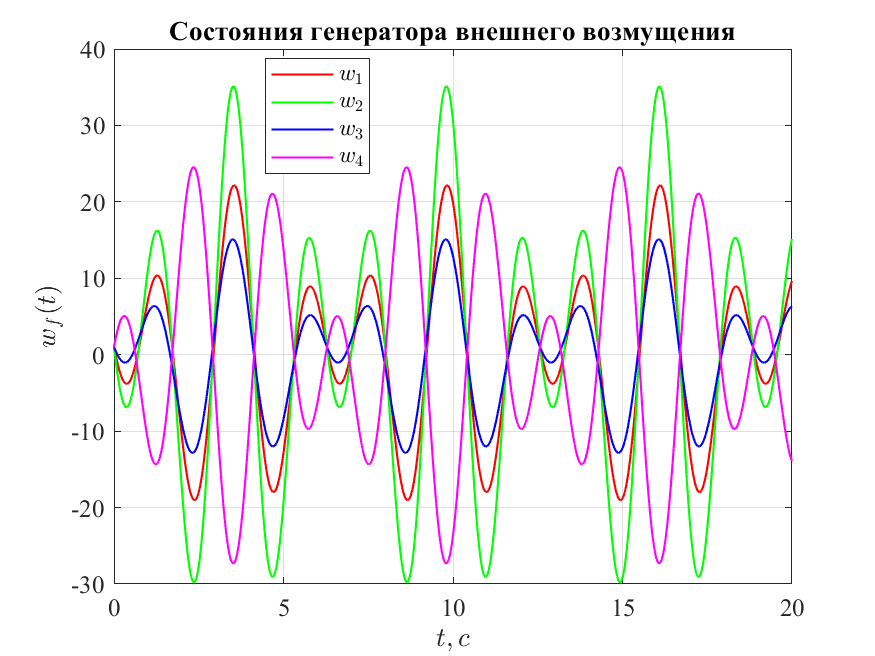
\includegraphics[width=0.8\textwidth]{w1.png}
  \caption{Моделирование - вектор состояния генератора внешнего возмущения}
\end{figure}

\begin{figure}[ht]
  \centering
  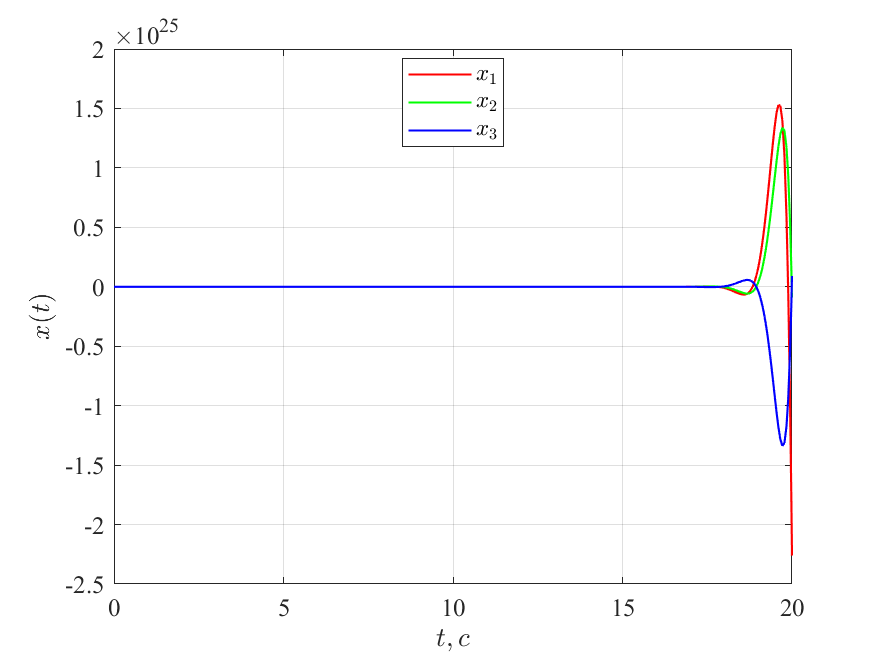
\includegraphics[width=0.8\textwidth]{x1.png}
  \caption{Моделирование - вектор состояния объекта управления}
\end{figure}

\begin{figure}[ht]
  \centering
  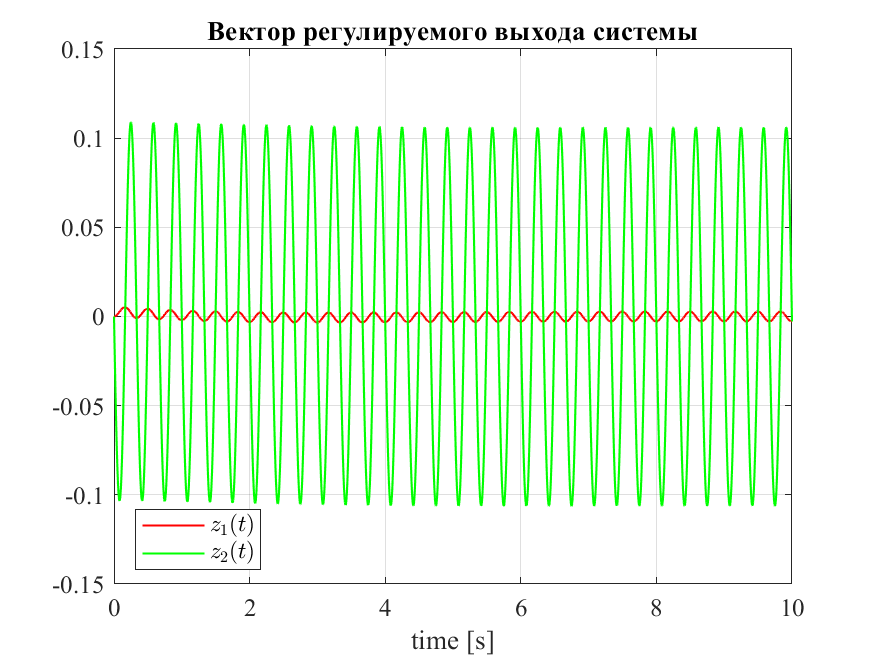
\includegraphics[width=0.8\textwidth]{z1.png}
  \caption{Моделирование - вектор виртуального выхода}
\end{figure}

Система изначально неустойчива, так как у неё есть неустойчивая мода, поэтому без управления вектора ничем не ограничены.

\newpage
\subsection{Замкнутая система, только с $K_1$}


\begin{figure}[ht]
  \centering
  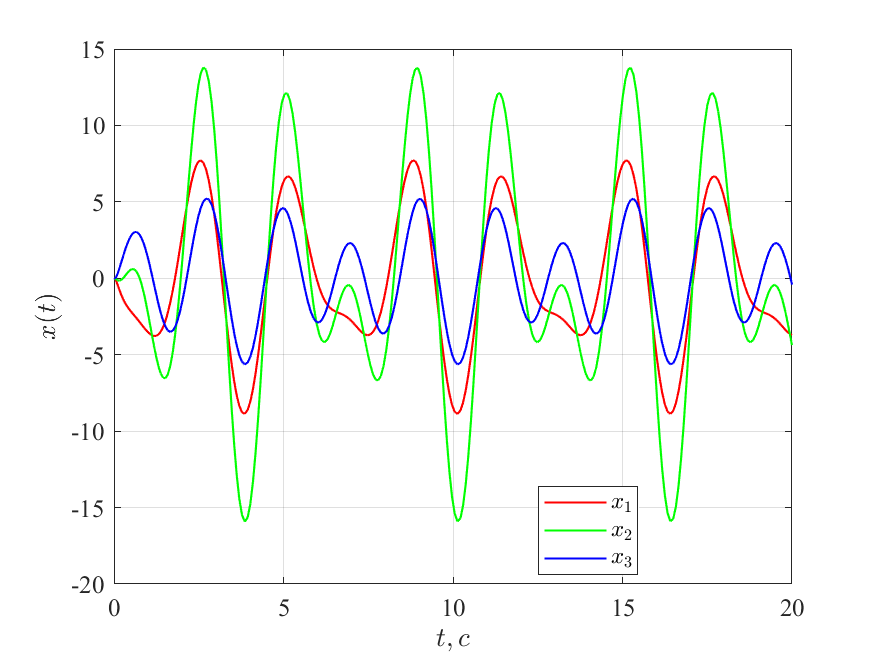
\includegraphics[width=0.8\textwidth]{x2.png}
  \caption{Моделирование - вектор состояния объекта управления}
\end{figure}

\begin{figure}[ht]
  \centering
  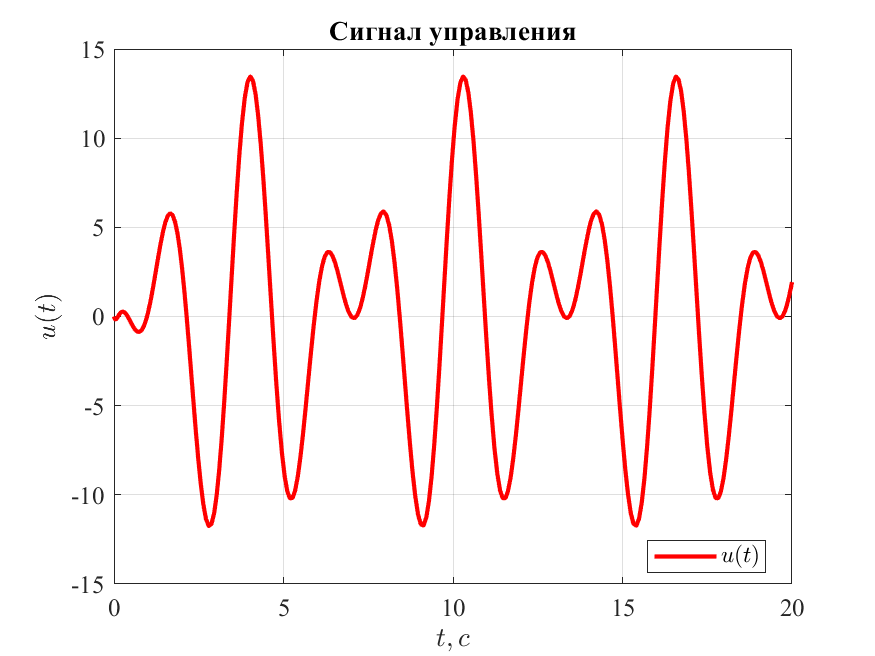
\includegraphics[width=0.8\textwidth]{u2.png}
  \caption{Моделирование - управляющий сигнал}
\end{figure}


\begin{figure}[ht]
  \centering
  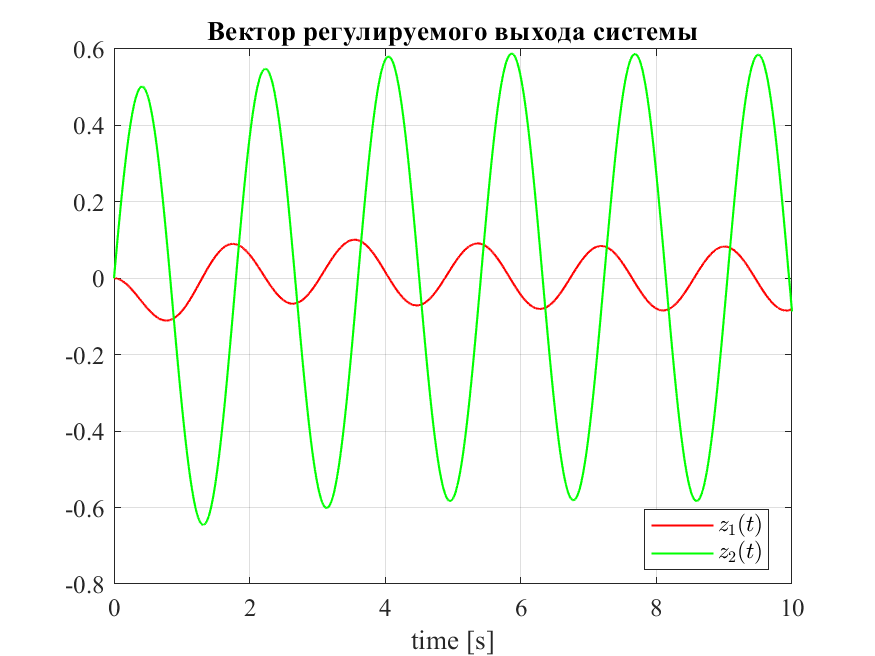
\includegraphics[width=0.8\textwidth]{z2.png}
  \caption{Моделирование - вектор виртуального выхода}
\end{figure}

Здесь ситуация улучшилась - система стала устойчива, но мы не решили задачу компенсации.
ром:

\newpage
\subsection{Полностью замкнутая система $(K_1 + K_2)$}

\begin{figure}[ht]
  \centering
  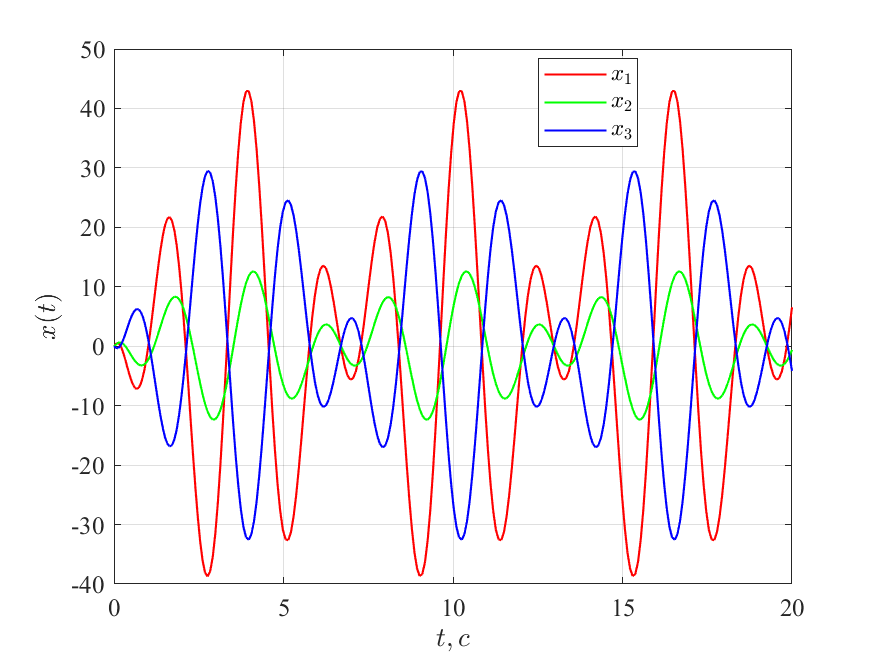
\includegraphics[width=0.8\textwidth]{x3.png}
  \caption{Моделирование - вектор состояния объекта управления}
\end{figure}

\begin{figure}[ht]
  \centering
  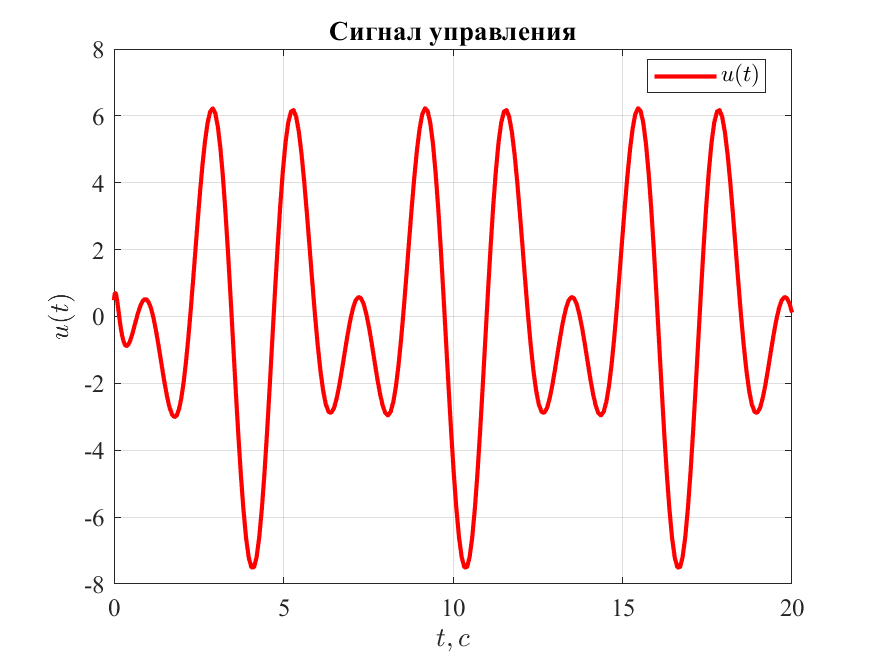
\includegraphics[width=0.8\textwidth]{u3.png}
  \caption{Моделирование - управляющий сигнал}
\end{figure}

\begin{figure}[ht]
  \centering
  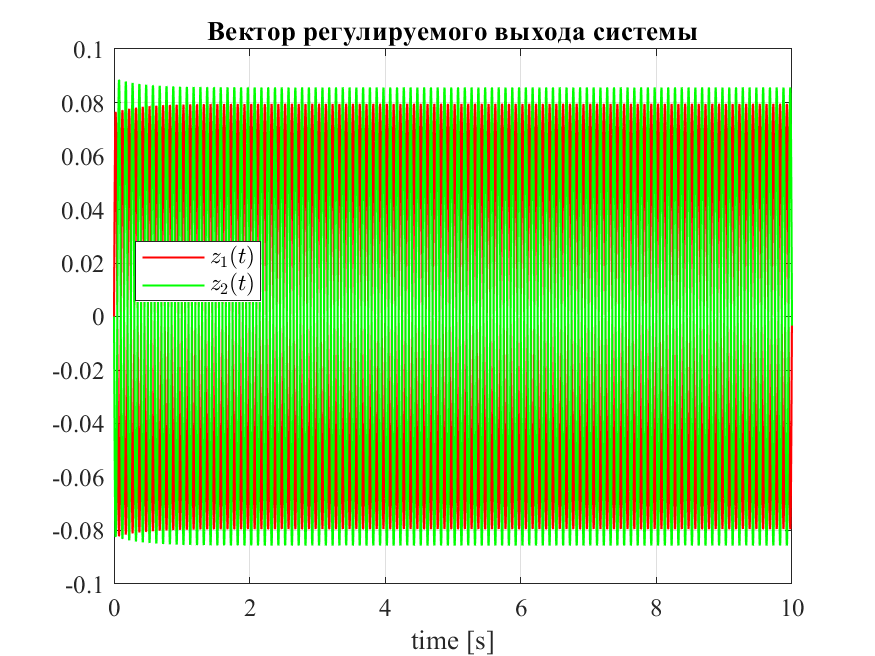
\includegraphics[width=0.8\textwidth]{z3.png}
  \caption{Моделирование - вектор виртуального выхода}
\end{figure}

Виртуальный выход системы сходится к нулю, задача компенсации решена.

\section{Выводы}

В этом задании мы синтезировали компенсирующий регулятор с помощью $LQR$ и решения матричного уравнения Ляпунова. 
Он состоит из feedback-компоненты,которая отвечает за стабилизацию системы,
и feedforward-компоненты, за счёт которой мы компенсируем динамику внешнего возмущения.

\endinput